\documentclass[a4paper, 12pt]{article}

\usepackage[left = 3cm, top = 3cm, bottom = 3cm, right = 2cm]{geometry}
\usepackage{graphicx}
\usepackage[spanish,es-tabla]{babel} % Idioma español con tablas
\usepackage{amsmath}
\usepackage{amssymb}
\usepackage{amsfonts}
\usepackage[utf8]{inputenc}         % Para escribir en castellano
\usepackage[T1]{fontenc}
\usepackage{color}
\usepackage{alltt}
\usepackage{times}
\usepackage{setspace}  % Usado para doble espacio, espacio y medio y espacio simple
\usepackage{booktabs}         % Para formar tablas
%\usepackage{longtable}       % Usado para diseñar grandes tablas.
\usepackage[round]{natbib} 
\bibliographystyle{apalike}

\usepackage[x11names,table]{xcolor}

\begin{document}

\begin{center}
 {\bf {\fontsize{14}{16.8}\selectfont UNIVERSIDAD NACIONAL DE TRUJILLO}}     
 
    {\bf{\fontsize{14}{16.8}\selectfont Facultad de Ciencias Físicas y Matemáticas}} 

  {\bf{\fontsize{14}{16.8}\selectfont Escuela Profesional de Informática}}
\end{center}  

\begin{figure}[ht]
\begin{center}

\includegraphics[width=.3\textwidth]{unt}
\end{center}
\end{figure}

\vskip 2cm
\begin{center}
  { \bf {\fontsize{17}{20.4}\selectfont{Desarrollo de un sistema BMS-IoT para el control automatizado del consumo eléctrico basado en el protocolo MQTT}}  } 
%\end{center}  

 
  \vskip 2cm
  { \bf {\fontsize{17}{20.4}\selectfont{\hspace*{-0.4cm}Autores: }}  }
  
 \vskip 0.25cm 
  
   Daniel I. Cruz Flores \\
   Leoncio M. Moya Carranza
 
	   
  \vskip 1cm
  { \bf {\fontsize{17}{20.4}\selectfont{\hspace*{-0.4cm}Asesor: } }  } 
 \vskip 0.25cm 
 
   Dra. Patricia Pereyra Salvador
  
\vskip 4cm


%\begin{center}    
{\bf {\fontsize{14}{16.8}\selectfont Trujillo - La Libertad
\vskip 0.0cm
\hspace*{-0.2cm} 
\vskip 0.1cm
2022 }}
\end{center} 
\newpage

\begin{center}
%\onehalfspace  \doublespacing  \singlespace
\Large {PROYECTO DE INVESTIGACIÓN PARA TRABAJO DE GRADUACIÓN \\
\vskip 0.2cm
 ESCUELA PROFESIONAL DE INFORMÁTICA}
\end{center}
\vskip 1cm

\section{GENERALIDADES}
%De acuerdo con  \cite{Erica} las investigaciones nacen de una idea, sin importar qué tipo de paradigma fundamente el estudio ni el enfoque que se habrá de seguir. Para dar inicio a la investigación se necesita primero, la idea que éste será el primer acercamiento a lo que realmente se quiere investigar o al ambiente al cual  habra que estudiar. \par
%\vskip 0.3cm
%La investigación es la realización de un trabajo de búsqueda, mediante el uso del método científico, para adquirir conocimientos científicos y describir, explicar y predecir los fenómenos que ocurren en esa pequeña parte de universo que se quiere estudiar y conocer.               



\subsection{Título}
Desarrollo de un sistema BMS-IoT para el control automatizado del consumo eléctrico basado en el protocolo MQTT.

\subsection{Autor(es)}
%Indicar apellidos y nombres de los participantes:
\begin{table}[h!]
 \caption{\small{Datos del alumno (s) investigador (es)}}
\begin{tabular}{llrrr} \toprule
{\bf Código(s)} & {\bf Nombres y Apellidos} & {\bf Cargo en el proyecto} & {\bf Email} \\ \midrule
512701004 & Daniel I. Cruz Flores & Investigador. & ivan17cf@gmail.com \\
022700305    & Leoncio M. Moya Carranza & Investigador. & leonciomoya@gmail.com            \\ \bottomrule
\end{tabular}
\end{table}



\subsection{Tipo de investigación}

\begin{itemize}
\item De acuerdo al fin que se persigue: Aplicada 
\item De acuerdo al alcance de  la investigación: Descriptiva experimental.
\end{itemize}



\subsection{Área y línea de Investigación}
\begin{itemize}
\item ÁREA DE INVESTIGACIÓN: redes y conectividad, lenguajes de programación orientado a objetos y sistemas embebidos.
\item LÍNEAS DE INVESTIGACIÓN: ingeniería de software, Redes de computadoras e Internet de las cosas.

\end{itemize}

               
\subsubsection{Tema de investigación :} 

El protocolo de red MQTT y su aplicación en soluciones IoT

\subsection{Localidad e Institución donde se desarrollará el proyecto }

\begin{itemize}

\item LOCALIDAD: 
Departamento de la Libertad, Provincia de Trujillo, distrito de Trujillo.

\item INSTITUCIÓN: 
Universidad Nacional de Trujillo / Facultad de ciencias físicas y matemáticas/ Informática.

\end{itemize}




  
\subsection{Duración del trabajo de graduación (Plan TG y desarrollo del TG)}
%Ejemplo:\\
\hspace*{0.7cm}Del \hspace*{0.2cm}15/07/2022 \hspace*{0.3cm} AL\hspace*{0.2cm}30/12/2022  \hspace*{0.2cm}(05 meses +  15 días)
  
    
  
  
\subsection{Cronograma del trabajo de graduación}


%\subsubsection{Cronograma del plan TG y avance del desarrollo TG (un ciclo) }

 \begin{table}[h!]
  \caption{\small{Etapas y actividades para el trabajo de graduación}}
\centering
\begin{tabular}{|p{3cm} |p{4cm} |p{2.2cm} |p{2.6cm} |p{2.3cm}|}  \hline   
\textit{{\bf{Etapas}}} & \textit{{\bf{Actividades/tareas}}} & \textit{{\bf{Fecha inicio}}} & \textit{{\bf{Fecha término}}} & \textit{{\bf{Hs. semanal}}}\\ \hline

Preparación del plan TG. & Elaborar plan TG.\par Aprob. plan TG.  & 10/11/2022\par 20/09/2016 & 05/05/2017\par 05/05/2017 & 4\par 1  \\ \hline
Recopilación de información. & Inv. bibliográfica.\par Instrumentos de medición. & 05/05/2017\vskip 0.5cm \par 05/05/2017  & 05/05/2017\vskip 0.5cm \par 05/05/2017 & 30\vskip 0.5cm\par 25    \\  \hline

Análisis de datos recolectados. & Procesamiento e interpretación de la información. &\vskip 0.2cm 05/05/2017 &\vskip 0.2cm 05/05/2017 & \vskip 0.2cm 10 \\ \hline

Resultados. & Desarrollo de TG segun cronograma. &\vskip 0.2cm 05/05/2017 &\vskip 0.2cm 05/05/2017 & \vskip 0.2cm 10 \\ \hline

Redacción del informe TG.  &Informe N1: Marco teórico y metodología. \par
Informe N2: Propuesta de solución al problema formulado.\par 
Informe N3: Resultados y conclusiones preliminares. &\vskip 0.2cm\par  05/05/2017\par \vskip 1.1cm \par 05/07/2017\par \vskip 0.9cm 05/08/2017 & \vskip 0.2cm\par  05/02/2017\par  \vskip 1.1cm 05/05/2017\par \vskip 0.9cm 05/06/2017 &  \vskip 0.2cm\par 50\par  \vskip 1.1cm\par 93\par \vskip 0.9cm 20                \\  \hline

Recopilación de información adicional para la tesis & Inv. bibliográfica adicional y su interpretación.  & 05/08/2016 & 05/05/2017 & 4  \\ \hline

Pruebas y análisis de resultados & Preparación de resultados finales.  & 05/08/2016 & 05/05/2017 & 4  \\ \hline


Redacción del informe de tesis & Informe de tesis de acuerdo con formato establecido.  & 05/08/2016 & 05/05/2017 & 4  \\ \hline
\end{tabular}
\begin{center}
\vskip -0.2cm
{\small{Fuente: Elaboración propia.}}
\end{center}
\end{table}




\subsection{Recursos disponibles}
\subsubsection{{\bf Personal:}} Personal técnico, administrativo y de servicios disponibles para el proyecto.
\subsubsection{ {\bf	Materiales y Equipos:}} Se debe especificar la calidad y cantidad de equipos, instrumentos y materiales disponibles  para ejecutar el trabajo de investigación.
\subsubsection{{\bf Locales:}} Señalar los ambientes donde se realizará la investigación: laboratorios, aulas, biblioteca, hemeroteca, etc.  indicando su ubicación precisa.

\subsection{Presupuesto}
Costear en nuevos soles, los bienes, servicios e inversiones necesarios para llevar a cabo la investigación y que no estén disponibles. Presentar ordenados de acuerdo a la codificación del  Clasificador de Gastos vigente. Considerar calidad, cantidad y  precio.

\subsection{Financiamiento}
\subsubsection{ {\bf	Con recursos universitarios:}}  Los recursos disponibles por subvención por investigación.
\subsubsection{ {\bf Con recursos externos:}} Los que se perciban de fuente distinta a la UNT. Indicar la entidad aportante y los montos.
\subsubsection{ {\bf Autofinanciación:}} Aporte del investigador (Puede ser en bienes o efectivo).




\section{PLAN DE INVESTIGACIÓN}
Es  parte del proyecto de Investigación,  debe ser lo suficientemente detallado para permitir comprender la naturaleza y los alcances de la investigación; así como, la rigidez del método seguido. Debe contener las citas bibliográficas (en norma APA) y estructurarse con  subtítulos de acuerdo los ítems siguientes:

\subsection{Realidad problemática}
Para la realización de una investigación, el equipo investigador debe ubicarse en la realidad problemática dentro de un campo de interés y resaltar su importancia. Considerar estadísticas e indicadores numéricos que describan la situación problemática de la realidad.

\subsection{Antecedentes}
% y fundamentación científica, técnica o humanística}
Para la realización de una investigación, el equipo investigador debe 
citar y comentar investigaciones recientemente realizadas que se relacionan con el problema o tema de investigación.
\vskip 0.3cm
{\bf Ejemplo de antecedente}: Cuando se expresa exactamente lo que dice el autor:\par
\vskip 0.3cm
\cite{Ghiani} entienden que la logística trata de la planificación y control de los flujos de materiales e informaciones relacionadas en las organizaciones, tanto en los sectores público y privado. Además su misión es hacer la entrega de los productos correctos, en el local correcto y en la hora correcta, optimizando los costos operacionales totales del proceso.
satisfaciendo un determinado conjunto de restricciones o condiciones.\par
\vskip 0.4cm
{\bf Ejemplo de antecedente}: Cuando se interpreta lo que dice el autor:\par

El desarrollo sustentable, (Figura 1), estará garantizado si se consideran tres aspectos fundamentales: económico, social y ambiental, donde la intersección de estos aspectos garantiza la calidad de vida en el espacio urbano y el equilibrio en las clases sociales en busca del bienestar \citep{Tanguay}.

\begin{figure}[ht]
\begin{center}
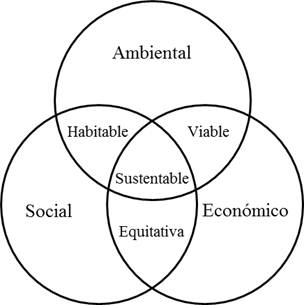
\includegraphics[width=0.3\textwidth]{Figura2}
\end{center}
\begin{center}
\vskip -0.5cm
\caption{\small{Aspectos claves para el desarrollo sustentable.}}
{\small{Fuente: \cite{Tanguay}}}
\end{center}
\end{figure}


\vskip 0.4cm
{\bf Otros ejemplos de antecedentes}: \par

En los años 90 se presentaron definiciones generales las cuales vienen siendo mejoradas. \cite{Dekker} presenta una mejora en la definición de logística reversa como  ”el proceso de planificación, implementación y control de los flujos de materias-primas, en procesos de inventarios y bienes acabados, desde el punto de fabricación, distribución o uso, hacia el punto de recuperación o de eliminación”. 


\begin{figure}[ht]
\begin{center}
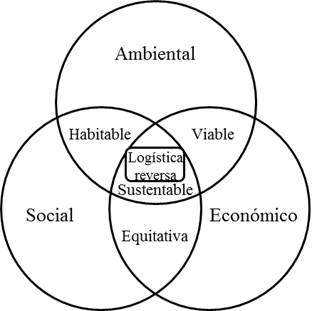
\includegraphics[width=0.3\textwidth]{Figura1}
\end{center}
\begin{center}
\vskip -0.5cm
\caption{\small{Logística reversa incluida en el desarrollo sustentable.}}
{\small{Fuente: Adaptación de \cite{Tanguay}}}
\end{center}
\end{figure}



\vskip 0.4cm
El problema de ruteo de vehículos \citep{Ombuki, Yeun} y sus variantes han ganado mucho interés en la comunidad académica. La intención de estar más cerca a la realidad mediante el modelamiento matemático, hace que se hayan desarrollado nuevos modelos de optimización. \par
\vskip 0.4cm
Según \cite{Sterle} el primer nivel de la red comprende la distribución de la carga desde las plataformas hasta las unidades satélites, utilizando vehículos de carga de mayor tamaño (g).  El segundo nivel, consiste en montar rutas desde las unidades satélites hasta los clientes, usando para este caso vehículos de menor tamaño (v). El modelo de localización y ruteo de vehículos para la distribución de carga propuesto por el autor, además de hacer la conexión de los dos niveles y estudiar su inter relación y dependencia, el modelo busca determinar la cantidad necesaria de plataforma y de unidades satélites considerando el tamaño y dimensionamiento de la flota para el ruteo en dos niveles. 
\vskip 0.2cm


\begin{table}[h!]
\begin{center}
\caption{\small{Resultados computacionales obtenidos en el modelo de \cite{Sterle}}}
\end{center}
\vskip -0.7cm
\begin{tabular}{cccc} \toprule %{|c|c|c|c|} \toprule
\hline 
\rowcolor{LightBlue2}{\small Escenarios} & {\small Demanda cliente (ton.)} & {\small Tiempo (min.)} & {\small Costo ($\$$)} \\ \hline 
{\small 1} & {\small P1:1; P2:2; P3:2; P4:2; P5:1} & {\small 0.12} & {\small 667.42} \\ \hline 
{\small 2} & {\small P1:1; P2:2; P3:2; P4:2; P5:1; P:4; P7:3} & {\small 56.54} & {\small 1744.35} \\ \hline 
{\small 3} & {\small P1: 1; P2:2; P3:2; P4:2; P5:1; P6: 4; P7:3; P8:2; P9:2} & {\small 287.70} & {\small 1750.72} \\  \hline 
{\small 4} & {\small P1:1; P2:2; P3: 2; P4:2; P5:1; P6:4; P7:3; P8:2; P9:2; P10:1} & {\small 1848.57} & {\small 1773.46} \\   \bottomrule \hline 
\end{tabular} 
\begin{center}
\vskip -0.2cm
{\small{Fuente: Resultados obtenidos con CPLEX.}}
\end{center}
\end{table}



\subsection{Justificación}
La mayoría de las investigaciones se efectúan con un propósito definido. Tal propósito debe ser lo suficientemente fuerte para que justifique su realización. \cite{Erica}  

\begin{enumerate}
\item[(a)] Razones o motivos e importancia del tema a ser investigado. 
\item[(b)]Sustentar la pertinencia de la pregunta o problema que se abordará en la investigación.
\item[(c)]Considerar los resultados esperados e impactos previstos.
\end{enumerate}


\subsection{Problema}
Plantear el problema no es otra cosa mas que afinar y estructurar formalmente la idea de investigación. El planteamiento del problema puede ser sencillo o complejo dependiendo de la familiarización del investigador en el tema a tratar.\par    
\vskip 0.3cm
Los criterios para formular un problema de investigación son:
\begin{enumerate}
\item[a)] El problema debe ser formulado claramente y sin ambiguedad como pregunta: ¿Qué efecto?; ¿en qué condiciones ...?; ¿cuál es la probabilidad de ...?; ¿cómo se relaciona ... con ...?; ¿cómo ...?.
\vskip 0.3cm
\item[b)] El planteamiento debe implicar la posibilidad de realizar una prueba empírica o una recolección de datos, es decir, la factibilidad de observarse en la realidad o en un entorno. 
\end{enumerate}
Por lo tanto, los elementos para plantear un problema de investigación son tres y estan relacionados entre si: Los objetivos que persigue la investigación; las preguntas de investigación y la justificación del estudio. \cite{Erica}
\vskip 0.3cm
{\bf Ejemplo:}\par  
¿Cómo viabilizar una red logística reversa en regiones urbanas minimizando los costos logísticos de ruteo y transporte de los RSU hasta su disposición final?


\subsection{Hipótesis}
Preferentemente para investigaciones explicativas debe ser una respuesta a priori y tentativa guardando coherencia con el problema científico, se formula como una proposición afirmativa, con un lenguaje claro y específico.  Las hipótesis se obtienen por deducción lógica y está sustentada en los conocimientos científicos. \par  
\vskip 0.3cm
{\bf Criterios para formular hipótesis:} \cite{Erica}
\begin{enumerate}
\item[a)] Toda hipótesis de investigación debe ser verificable estadísticamente.  Puede ser difícil o imposible de verificar porque no existe un conocimiento sobre el cual se pueda formular una hipótesis, o bien, porque una o más variables no son medibles.
\vskip 0.2cm
\item[b)] Toda hipótesis debe indicar la relación entre variables, lo que implica que las variables deben ser medibles.
\vskip 0.2cm
\item[c)] Toda hipótesis debe tener sus límites. Pueden escogerse hipótesis que sean sencillas de validar, y sin embargo, altamente significativas.
\vskip 0.2cm
\item[d)] El investigador debe tener una razón específica para considerar una hipótesis, ya sea teórica o por alguna evidencia concreta.    
\end{enumerate}


\subsection{Variables}
Las hipótesis consideran una relación entre dos elementos. A estos elementos se les llama variables. Las variables son los atributos que se miden en las hipótesis. Son factores que explican los resultados y determinan las diferencias entre éstos para poder establecer comparaciones. Son los elementos que se relacionan en una hipótesis. \cite{Erica} \par 
\vskip 0.2cm  
\subsubsection{Variable independiente}
Es el elemento que actua sobre el otro factor, al que se le denomina variable dependiente.

\subsubsection{Variables dependiente}
Variable que depende de la variable independiente.
\vskip 0.4cm

{\bf Ejemplo:} \cite{Erica}\par 
\vskip 0.2cm
{\bf Hipótesis:} Existe un mayor número de plantas comestibles en climas cálidos que en climas fríos. \par 
\vskip 0.2cm
Los elementos que se estan relacionando son: \par 
\begin{enumerate}
\item [(1)] plantas comestibles
\item[(2)] climas cálidos
\item[(3)] climas fríos
\end{enumerate} 
Estos tres elementos son variables. Por lo tanto:

{\bf Variable independientes:} Los climas.
\vskip 0.2cm

{\bf Variable dependiente:} Plantas comestibles.
\vskip 0.3cm
Para el caso de las investigaciones de alcanze explicativo, de la hipótesis se derivan las variables independiente(s) y dependiente.\par
\vskip 0.3cm
Para el caso de las investigaciones de alcanze descriptivo, al ser la hipótesis implícita solo se consideraran variables de investigación.\par
\vskip 0.3cm


\subsection{Objetivos}
Es necesario establecer qué pretende la investigación, es decir, cuáles son sus objetivos. Hay investigaciones que buscan contribuir a resolver un problema en especial, y otras tienen como objetivo principal probar una teoría o aportar evidencia empírica en favor de ella. \par 
\vskip 0.3cm
Segun \cite{Rojas}, los objetivos tienen que expresarse con claridad para evitar posibles desviaciones en el proceso de investigación y deben ser susceptibles de alcanzarse; son las guías del estudio y hay que tenerlos presentes durante todo su desarrollo. Los objetivos deben ser congruentes entre sí.
\vskip 0.3cm
Describir el objetivo central o propósito del proyecto de investigación (debe estar alineado con el problema e hipótesis), así como los objetivos específicos, los cuales deben reflejar los cambios que se esperan lograr en trabajo de tesis (variables). Para estos objetivos específicos utilice verbos como: describir, indicar, modificar, controlar, producir (tecnologías), recuperar, etc..

\subsubsection{Objetivos generales}
Debe explicitar lo que se espera lograr con el estudio en términos de conocimiento. Debe dar una noción clara de lo que se pretende describir, determinar, identificar, comparar y verificar.


\subsubsection{Objetivos específicos}
Son la descomposición y secuencia lógica del objetivo general. Son un anticipo del diseño de la investigación.
\vskip 0.3cm


{\bf Ejemplo de objetivos:}\\
%\vskip 0.1cm
{\bf Objetivo General:}
\begin{enumerate}
\item[a)] La investigación tiene como objetivo principal modelar y planificar una red logística reversa para una región urbana, dimensionando el flujo de RSU que será transportado a lo largo de la red y determinar el número y capacidad de las estaciones de colecta y de la unidades productivas y especiales necesarias para la atención de la región, en cuanto a la colecta, transporte y disposición final de los RSU.
\vskip 0.3cm
\item[b)]Con la optimización del modelo de colecta de RSU, es posible reorganizar el sistema logístico reverso de una ciudad de forma que se consiga un mejor dimensionamiento de la red, con la consecuente disminución del número que circulan en la ciudad.

\end{enumerate}
\vskip 0.2cm
{\bf Objetivos específicos:}
\begin{enumerate}
\item[a)] Aplicar una metodología de programación lineal entera, considerada computacionalmente como un problema que pertenece a la clase de complejidad NP \citep{Korte} para solucionar el problema.
\item[b)] Implementar con CPLEX, rodando en el sistema operativo Linux, los modelos propuestos, validarlos y testarlos en un caso práctico.

\end{enumerate}



\subsection{Método de trabajo}
De acuerdo con \cite{Erica}, para el desarrollo del método debe presentarse un bosquejo de la manera  en que se propone llevar a cabo la investigación, es decir, el camino a seguir o los pasos a seguir para realizar una cosa. Cuando mas complejo sea el bosquejo  más fácil se desarrollará el proceso de investigación. Se utiliza el vocablo método en vez de metodología, ya este último se considera equivocado, en el sentido en que se le utiliza comúnmente en informes de investigación. 
\vskip 0.3cm
Los tipos de métodos a usar para TG en informática, elegir un método, se considera:
\begin{enumerate}
\item[a)] {\bf Método deductivo:} Es un método de razonamiento que consiste en tomar conclusiones generales para explicaciones partículares. El método se inicia con el análisis de los postulados, teoremas, leyes, principios, etc., de aplicación universal y de comprobada validez, para aplicarlos  a soluciones o hechos particulares. 

\item[b)]{\bf Método cuantitativo:} Se fundamenta en la medición de las características de los fenómenos, lo cual supone derivar de un marco conceptual pertinente al problema analizado, una serie de postulados que expresen relaciones entre las variables estudiadas de forma deductiva, es decir, estudia fenómenos susceptibles de cuantificación y utiliza pruebas estadísticas para el análisis de datos. Este método tiende a generalizar y normalizar resultados. 

\item[c)] {\bf Método inductivo:} Se utiliza el razonamiento para obtener conclusiones que parten de hechos particulares aceptados como válidos, para llegar a conclusiones, cuya aplicación sea de caracter general. El método se inicia con un estudio individual de los hechos y se formulan conclusiones universales que se postulan como leyes, principios o fundamentos de una teoría.

\item[d)] {\bf Análisis y sintesis:} Estudia los hechos, partiendo de la descomposición del objeto de estudio en cada una de sus partes para estudiarlas en forma individual (análisis), y luego se integran dichas partes para estudiarlas de manera holística e integral (síntesis).
\end{enumerate}

Por lo tanto, plantear el objeto de estudio, el diseño de investigación a usar, las técnicas de recolección de la información a ser utilizadas, definir la población y tamaño de la muestra que debe ser representativa y necesaria para hacer generalizaciones, {\bf etapas del estudio} y análisis estadístico. El método de estudio entre otras cosas se refiere a la secuencia de pasos que se sigue para alcanzar los objetivos trazados, considerando los métodos propuestos anteriormente.\par
\vskip 0.3cm
{\bf Ejemplo:}\par
\vskip 0.1cm
Para llegar a los objetivos propuestos, el desarrollo de la investigación comprendió las siguientes etapas de trabajo a saber:
\begin{enumerate}
\item[a)] Análisis del problema de gestión de residuos sólidos urbanos (RSU) en el Brasil, para comprender la situación actual y levantar los principales cuellos de botella. Además, definir las principales variables de decisión para el modelamiento;
\item[b)]	Levantamiento de los principales casos de éxito en la gestión de RSU en las ciudades brasileras, peruanas y de otros países;  
\item[c)]	Formulación del problema principal de la investigación, justificando su importancia;
\item[d)]	Levantamiento bibliográfico de los diferentes temas necesarios para la elaboración de la investigación, tales como Leyes de RSU, sustentabilidad, ruteo, logística urbana, logística reversa y gestión de residuos, entre otros;
\item[e)]	Estudio y análisis de los modelos de ruteo, logística urbana y logística reversa que contribuyan con el estado de arte del problema formulado;
\item[f)]	Estudio y análisis de los métodos de solución para resolver los modelos evaluados en la revisión bibliográfica, así como los modelos que serán propuestos en este estudio;
\item[g)]	Investigación y estudio de software libre que permita el teste de los modelos estudiados y la implementación de los modelos desarrollados en la investigación;
\item[h)]	Testes y validación de los modelos estudiados con la herramienta computacional escogida;
\item[i)]	Planificación del sistema de logística reversa para la sustentabilidad en el contexto de la logística urbana, por medio del desarrollo del modelamiento matemático del Sistema de Colecta Selectiva (ruteo) y de Transporte de los RSU hacia los centros especializado para que sean reciclados, reutilizados o rechazados;
\item[j)]	Elección de un área urbana para que sea utilizada como estudio de caso,  tanto para los testes de los modelos estudiados como de los modelos desarrollados;
\item[k)]	Levantamiento de los datos necesarios para validar y testar los modelos junto a los organismos responsables y organizaciones que participan directa e indirectamente en este campo de trabajo;
\item[l)]	Levantamiento de premisas y simulación de datos para ejecutar los programas, es decir, muchas veces las bases de datos reales que se encuentran son incompletas y por un determinado dato no se puede ejecutar el programa, en este caso, esas informaciones son llenadas por medio de simulaciones de datos considerando la experiencia del analista de sistemas;
\item[m)]	Testes y validación de los modelos desarrollados en la ciudad escogida por medio de la generación de escenarios alternativos.    
\end{enumerate}
    



\subsection{Referencias}
Presentar bibliografía conforme a las normas técnicas internacionales reconocidas: Un solo estilo American Psychological Association - APA. Seguir exactamente la forma de las referencias dadas como ejemplos. No usar numeros entre corchetes. Ver los ejemplos de las referencias dadas abajo.\par
\vskip 0.3cm
Se exige como mínimo 10 referencias entre libros y/o artículos referentes al tema a investigar. Las referencias sustentan la investigación del TG.

\bibliography{Bibliografia} % Bibliografia formato APA


\vskip 1cm

\hspace{0.7cm}Daniel\hspace{.1cm}I.\hspace{.1cm} Cruz\hspace{.1cm}Flores 
\hspace{4cm}Leoncio\hspace{.1cm}M.\hspace{.1cm} Moya\hspace{.1cm}Carranza \\
\hspace*{2.6cm} Alumno  \hspace*{6.6cm}Alumno


\vskip 1cm
\begin{center}
Dra. \hspace{.1cm}Patricia\hspace{.1cm} Pereyra\hspace{.1cm}Salvador\\
 Asesor
\end{center}



\end{document}

